\section{其他常见函数}
\subsection{单位阶跃函数}
\begin{definition}
函数\[
f(x) = \left\{ \begin{array}{cc}
0, & x < 0, \\
1, & x \geq 1
\end{array} \right.
\]称为\DefineConcept{单位阶跃函数}或\DefineConcept{赫维赛德阶跃函数}.
\end{definition}

\begin{figure}[htb]
	\centering
	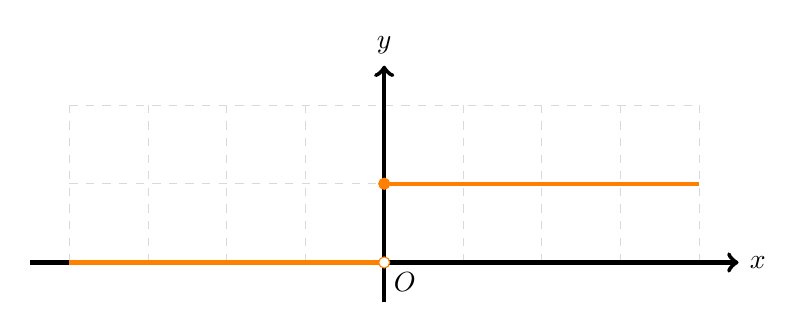
\begin{tikzpicture}
		\draw[help lines,color=gray!30,dashed](-4,0)grid(4,2);
		\draw[->,ultra thick](-4.5,0)--(4.5,0)node[right]{\(x\)};
		\draw[->,ultra thick](0,-.5)--(0,2.5)node[above]{\(y\)};
		\draw (0,0)node[below right]{\(O\)};
		\draw[orange,ultra thick](-4,0)--(0,0) (0,1)--(4,1);
		\draw[draw=orange,fill=orange](0,1)circle(2pt);
		\draw[draw=orange,fill=white](0,0)circle(2pt);
	\end{tikzpicture}
	\caption{单位阶跃函数的图形}
\end{figure}

\subsection{克罗内克\texorpdfstring{\(\delta\)}{\textdelta}函数}
\begin{definition}
%@see: https://mathworld.wolfram.com/KroneckerDelta.html
定义:\[
\delta_K(a,b)
\defeq \left\{ \begin{array}{cl}
	1, & a = b, \\
	0, & a \neq b.
\end{array} \right.
\]称其为\DefineConcept{克罗内克\(\delta\)函数}.
\end{definition}

\subsection{狄拉克\texorpdfstring{\(\delta\)}{\textdelta}函数}
\begin{definition}
%@see: https://functions.wolfram.com/GeneralizedFunctions/DiracDelta/02/
%@see: https://functions.wolfram.com/GeneralizedFunctions/DiracDelta2/02/
定义:\[
	\delta_D(x)
	\defeq \frac{1}{\pi}
		\lim_{\epsilon\to0}
		\frac{\epsilon}{x^2+\epsilon^2}
	\quad(x\in\mathbb{R}).
\]
称其为\DefineConcept{狄拉克\(\delta\)函数}.
\end{definition}

%@see: https://mathworld.wolfram.com/DeltaFunction.html
